%
%
%

\begin{frame}[t]{The perceptron}

    The \index{perceptron}\gls{perceptron} 
    is the simplest \index{neural network}neural network:
    It contains {\bf a single input layer} and {\bf an output node}.\\
    \vspace{0.2cm}
    It is a
    \index{binary classification}{\bf binary classification} algorithm for 
    \index{supervised learning}{\bf supervised learning}.

    \begin{center}
        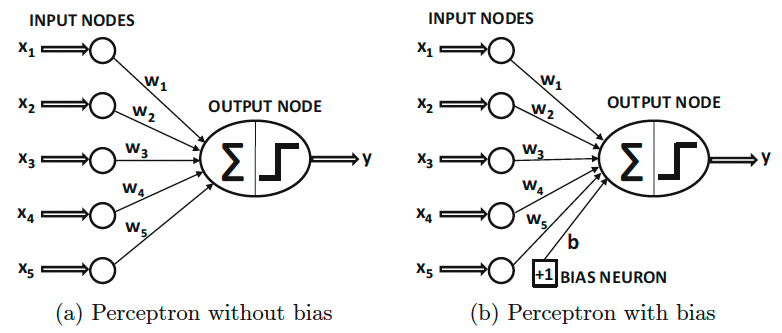
\includegraphics[width=1.00\textwidth]{./images/perceptron/basic_architecture.png}\\
        \vspace{-0.2cm}
        {\scriptsize \color{col:attribution} 
        Basic architecture of the Perceptron. 
        Image reproduced from p.5 of \cite{Aggarwal:2018SpringerDL}}\\
    \end{center}

\end{frame}


%
%
%

\begin{frame}[t]{What function does the perceptron compute?}

    Let $\hat{y}$ be our prediction of $y$ for a given feature vector $\vect{x}$.
    The \index{perceptron}\gls{perceptron} computes the prediction as follows:
    \begin{equation}
        \hat{y} = sign\Big\{ \vect{w}^T \cdot \vect{x} \Big\} = sign\Big\{ \sum_{i=1}^{d} w_i x_i \Big\}
        \label{eq:perceptron_prediction_wo_bias}
    \end{equation}        

    \vspace{-1.0cm}

    \begin{columns}
        \begin{column}{0.50\textwidth}
         \begin{center}
          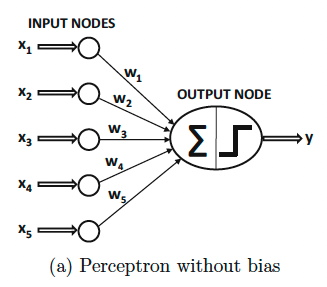
\includegraphics[width=0.95\textwidth]{./images/perceptron/perceptron_without_bias.png}\\
          {\scriptsize \color{col:attribution} 
          Image reproduced from p.5 of \cite{Aggarwal:2018SpringerDL}}\\
         \end{center}
        \end{column}
        \begin{column}{0.50\textwidth}
            \begin{itemize}
                \small
                \item Computes a linear function 
                ($\vect{w}^T \cdot \vect{x}$) in the output node.
                \item The sign function plays the role of
                an \index{activation function}\gls{activation function}.
                \item It maps a real value to either +1 or -1.
            \end{itemize}        
        \end{column}
    \end{columns}
      
\end{frame}

%
%
%

\begin{frame}[t]{What function does the perceptron compute?}

    We may need to add a \index{bias}{\bf bias} variable $b$, 
    to capture an invariant part of the prediction. 
    In this case, the \index{perceptron}\gls{perceptron} prediction is computed as follows:
    \begin{equation}
        \hat{y} = 
            sign\Big\{ \vect{w}^T \cdot \vect{x} + b \Big\} = 
            sign\Big\{ \sum_{i=1}^{d} w_i x_i + b \Big\}
            \label{eq:perceptron_prediction_w_bias}    
    \end{equation}

    \vspace{-1.0cm}

    \begin{columns}
        \begin{column}{0.50\textwidth}
         \begin{center}
            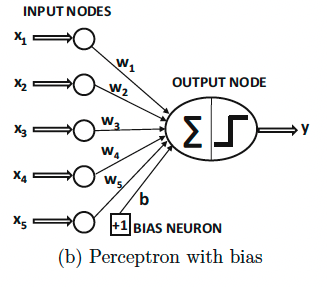
\includegraphics[width=0.95\textwidth]{./images/perceptron/perceptron_with_bias.png}\\
            {\scriptsize \color{col:attribution} 
            Image reproduced from p.5 of \cite{Aggarwal:2018SpringerDL}}\\
         \end{center}
        \end{column}
        \begin{column}{0.50\textwidth}
            \begin{itemize}
                \small
                \item Another approach to incorporate the bias, 
                is by \index{feature engineering}\gls{feature engineering}.
                \item Bias is the weight applied to an additional ($d$+1) 
                feature variable that always takes the value of 1.
                \item With that additional feature variable, 
                Eq. \ref{eq:perceptron_prediction_w_bias}
                can be reduced to Eq. \ref{eq:perceptron_prediction_wo_bias}.
                Therefore, for simplicity, will not show the bias explicitly.
            \end{itemize}        
        \end{column}
      \end{columns}

\end{frame}

